\documentclass[]{book}
\usepackage{lmodern}
\usepackage{amssymb,amsmath}
\usepackage{ifxetex,ifluatex}
\usepackage{fixltx2e} % provides \textsubscript
\ifnum 0\ifxetex 1\fi\ifluatex 1\fi=0 % if pdftex
  \usepackage[T1]{fontenc}
  \usepackage[utf8]{inputenc}
\else % if luatex or xelatex
  \ifxetex
    \usepackage{mathspec}
  \else
    \usepackage{fontspec}
  \fi
  \defaultfontfeatures{Ligatures=TeX,Scale=MatchLowercase}
\fi
% use upquote if available, for straight quotes in verbatim environments
\IfFileExists{upquote.sty}{\usepackage{upquote}}{}
% use microtype if available
\IfFileExists{microtype.sty}{%
\usepackage{microtype}
\UseMicrotypeSet[protrusion]{basicmath} % disable protrusion for tt fonts
}{}
\usepackage[margin=1in]{geometry}
\usepackage{hyperref}
\hypersetup{unicode=true,
            pdftitle={Reproducible Templates (Book in Development)},
            pdfauthor={Melinda K. Higgins},
            pdfborder={0 0 0},
            breaklinks=true}
\urlstyle{same}  % don't use monospace font for urls
\usepackage{natbib}
\bibliographystyle{apalike}
\usepackage{longtable,booktabs}
\usepackage{graphicx,grffile}
\makeatletter
\def\maxwidth{\ifdim\Gin@nat@width>\linewidth\linewidth\else\Gin@nat@width\fi}
\def\maxheight{\ifdim\Gin@nat@height>\textheight\textheight\else\Gin@nat@height\fi}
\makeatother
% Scale images if necessary, so that they will not overflow the page
% margins by default, and it is still possible to overwrite the defaults
% using explicit options in \includegraphics[width, height, ...]{}
\setkeys{Gin}{width=\maxwidth,height=\maxheight,keepaspectratio}
\IfFileExists{parskip.sty}{%
\usepackage{parskip}
}{% else
\setlength{\parindent}{0pt}
\setlength{\parskip}{6pt plus 2pt minus 1pt}
}
\setlength{\emergencystretch}{3em}  % prevent overfull lines
\providecommand{\tightlist}{%
  \setlength{\itemsep}{0pt}\setlength{\parskip}{0pt}}
\setcounter{secnumdepth}{5}
% Redefines (sub)paragraphs to behave more like sections
\ifx\paragraph\undefined\else
\let\oldparagraph\paragraph
\renewcommand{\paragraph}[1]{\oldparagraph{#1}\mbox{}}
\fi
\ifx\subparagraph\undefined\else
\let\oldsubparagraph\subparagraph
\renewcommand{\subparagraph}[1]{\oldsubparagraph{#1}\mbox{}}
\fi

%%% Use protect on footnotes to avoid problems with footnotes in titles
\let\rmarkdownfootnote\footnote%
\def\footnote{\protect\rmarkdownfootnote}

%%% Change title format to be more compact
\usepackage{titling}

% Create subtitle command for use in maketitle
\newcommand{\subtitle}[1]{
  \posttitle{
    \begin{center}\large#1\end{center}
    }
}

\setlength{\droptitle}{-2em}
  \title{Reproducible Templates \emph{(Book in Development)}}
  \pretitle{\vspace{\droptitle}\centering\huge}
  \posttitle{\par}
  \author{Melinda K. Higgins}
  \preauthor{\centering\large\emph}
  \postauthor{\par}
  \predate{\centering\large\emph}
  \postdate{\par}
  \date{2018-01-21}

\usepackage{booktabs}
\usepackage{makeidx}
\makeindex
\usepackage[nottoc]{tocbibind}

\usepackage{amsthm}
\newtheorem{theorem}{Theorem}[chapter]
\newtheorem{lemma}{Lemma}[chapter]
\theoremstyle{definition}
\newtheorem{definition}{Definition}[chapter]
\newtheorem{corollary}{Corollary}[chapter]
\newtheorem{proposition}{Proposition}[chapter]
\theoremstyle{definition}
\newtheorem{example}{Example}[chapter]
\theoremstyle{definition}
\newtheorem{exercise}{Exercise}[chapter]
\theoremstyle{remark}
\newtheorem*{remark}{Remark}
\newtheorem*{solution}{Solution}
\begin{document}
\maketitle

{
\setcounter{tocdepth}{1}
\tableofcontents
}
\listoftables
\listoffigures
\chapter*{Preface}\label{preface}
\addcontentsline{toc}{chapter}{Preface}

This should be s short 2-3 paragraph summary of the book, what it is
about and such.

\section*{Why read this book}\label{why-read-this-book}
\addcontentsline{toc}{section}{Why read this book}

This should cover the purpose of the book and what the read will gain
after reading the book.

Include who this book is for - having some previous experience with R is
helpful, but a raw beginner could read these book - but it is assumed
that the reader knows how to install software on their computer, connect
to the Internet, find, create, copy and move files and folders on their
computer. some previous experience working with document and
presentation software like Word, google docs, open office, powerpoint,
others xxxxxx\ldots{}

Include things like:

\begin{itemize}
\tightlist
\item
  coursera course
\item
  filling in the gaps
\item
  seemingly disconnected applications brought together with rmarkdown
  glue
\end{itemize}

\section*{Structure of the book}\label{structure-of-the-book}
\addcontentsline{toc}{section}{Structure of the book}

A verbal summary of what is in the book, each capte or section,
organization and workflow - does it have to be sequential or can the
reader jump around as needed - have to reads versus optional
reads\ldots{}

\section*{Software information and
conventions}\label{software-information-and-conventions}
\addcontentsline{toc}{section}{Software information and conventions}

Software assumptions, workflow and style conventions used in book. Maybe
include stuff here on hints, warnings, and such.

\section*{Acknowledgments}\label{acknowledgments}
\addcontentsline{toc}{section}{Acknowledgments}

People to thank:

\begin{itemize}
\tightlist
\item
  emory, cfde, tnt team
\item
  coursera
\item
  chester ismay - fivethirtyeight package and feedback
\item
  yihui xie - online help and guidance with bookdown
\item
  developers of R, Rstudio, rmarkdown, bookdown, knitr, \ldots{}
\end{itemize}

\section*{Prerequisites}\label{prerequisites}
\addcontentsline{toc}{section}{Prerequisites}

Placeholder for now - maybe come back and add details on getting started
- what assumptions are made for getting setup to work thriugh the
exercises in this book - to get the full experience\ldots{}

See more in the ``Getting Started'' Chapter \ref{getstarted}.

\begin{center}\rule{0.5\linewidth}{\linethickness}\end{center}

This is a \emph{sample} book written in \textbf{Markdown}. You can use
anything that Pandoc's Markdown supports, e.g., a math equation
\(a^2 + b^2 = c^2\).

The \textbf{bookdown} package can be installed from CRAN or Github:

Remember each Rmd file contains one and only one chapter, and a chapter
is defined by the first-level heading \texttt{\#}.

To compile this example to PDF, you need to install XeLaTeX.

\section*{Colophon}\label{colophon}
\addcontentsline{toc}{section}{Colophon}

\subsection*{R Packages Used in This
Book}\label{r-packages-used-in-this-book}
\addcontentsline{toc}{subsection}{R Packages Used in This Book}

This book will use the \texttt{R} programming language \citep{R-base}
with the following \texttt{R} packages:

\begin{enumerate}
\def\labelenumi{\arabic{enumi}.}
\tightlist
\item
  \texttt{bookdown} \citep{R-bookdown}
\item
  \texttt{rmarkdown} \citep{R-rmarkdown}
\item
  \texttt{knitr} \citep{R-knitr}
\item
  \texttt{dplyr} \citep{R-dplyr}
\item
  \texttt{ggplot2} \citep{R-ggplot2}
\item
  \texttt{printr} \citep{R-printr}
\item
  \texttt{fivethirtyeight} \citep{R-fivethirtyeight}
\end{enumerate}

Other external refs, book \citep{xie2015}, and the FAD ref
\citep{Miller_Epstein_Bishop_Keitner_1985}.

\subsection*{R Session Info as of 2018-01-21
08:32:25}\label{r-session-info-as-of-2018-01-21-083225}
\addcontentsline{toc}{subsection}{R Session Info as of 2018-01-21
08:32:25}

This book was compiled using the \texttt{R} packages \texttt{bookdown},
\texttt{rmarkdown}, and \texttt{knitr} running under the following
\texttt{sessionInfo()}:

\begin{verbatim}
## R version 3.4.3 (2017-11-30)
## Platform: x86_64-w64-mingw32/x64 (64-bit)
## Running under: Windows 10 x64 (build 15063)
## 
## Matrix products: default
## 
## locale:
## [1] LC_COLLATE=English_United States.1252 
## [2] LC_CTYPE=English_United States.1252   
## [3] LC_MONETARY=English_United States.1252
## [4] LC_NUMERIC=C                          
## [5] LC_TIME=English_United States.1252    
## 
## attached base packages:
## [1] stats     graphics  grDevices utils     datasets  methods   base     
## 
## other attached packages:
## [1] fivethirtyeight_0.3.0 printr_0.1            ggplot2_2.2.1        
## [4] dplyr_0.7.4           knitr_1.18            rmarkdown_1.8.5      
## [7] bookdown_0.5.10      
## 
## loaded via a namespace (and not attached):
##  [1] Rcpp_0.12.13     rstudioapi_0.7   bindr_0.1        magrittr_1.5    
##  [5] munsell_0.4.3    colorspace_1.3-2 R6_2.2.2         rlang_0.1.4     
##  [9] plyr_1.8.4       stringr_1.2.0    tools_3.4.3      grid_3.4.3      
## [13] gtable_0.2.0     htmltools_0.3.6  lazyeval_0.2.0   yaml_2.1.16     
## [17] rprojroot_1.3-2  digest_0.6.12    assertthat_0.2.0 tibble_1.3.4    
## [21] bindrcpp_0.2     glue_1.1.1       evaluate_0.10.1  stringi_1.1.5   
## [25] compiler_3.4.3   scales_0.5.0     backports_1.1.1  pkgconfig_2.0.1
\end{verbatim}

\chapter*{About the Author}\label{about-the-author}
\addcontentsline{toc}{chapter}{About the Author}

Melinda Higgins has dual degrees in Chemometrics (PhD) and Statistics
(MS) with 25 years experience in research, teaching, consulting,
directing and managing projects. Her expertise includes
programming/scripting languages (R, S, Pascal, Perl, Prolog) and
statistical, mathematical, imaging, and geo-spatial processing software
packages (R, SAS, SPSS, MATLAB, SYSTAT, ENVI, ESRI ArcView, IMAGINE).
While at Georgia Tech Research Institute (1994-2011), she coordinated
large team projects with rigorous timelines, milestone tracking and
version control in the areas of remote sensing, geospatial information
systems, sensor fusion and target recognition. In her current work at
Emory (2007 --), she has 10+ yr expertise mentoring students and faculty
in nursing and public health science research and scholarship. Her
health research experience includes pattern recognition, phenotype
characterizations and longitudinal modeling in heart failure, diabetes,
cognitive impairment, and HIV/AIDS chronic disease populations.

\part{Part One}\label{part-part-one}

\chapter{History \& Exemplars}\label{history}

\section{Reproducible Research}\label{reproducible-research}

So why is reproducible research important and incredibly beneficial?
Let's take a look at its beginnings to find the answer.

In the early '90s, a geophysicist named Jon Claerbout revised his book
Earth Soundings Analysis with a valid complaint. He claimed that few
published results are reproducible in any practical sense. To verify
them requires almost as much effort as it took to create them in the
first place. After a time, even the authors are often unable to
reproduce their own results! For these reasons, many people ignore most
of the literature.

Then, in 1996, the Consolidated Standards of Reporting Trials (or
CONSORT) published a set of guidelines to fix problems that developed
from inadequate reporting of randomized controlled trials. Following
their lead, in 2004, the International Committee of Medical Journal
Editors stated they wouldn't publish a clinical trial that had not been
registered, and that they would only endorse registries meeting several
key criteria, including that they must be:

\begin{itemize}
\tightlist
\item
  free and publicly accessible,
\item
  open to all prospective registrants,
\item
  managed by a non-profit organization, and
\item
  electronically searchable and validated
\end{itemize}

As a result of this turmoil in validity and research, the Food and Drug
Administration got on board and required the registration of even more
clinical trials. The Journal of Biostatistics also encouraged
reproducible practices of author submissions. They began marking
accepted papers based on the standards of reproducibility that were
followed. For example, papers marked with a `D' marking meant the data
on which the study is based is freely available. A `C' marking means the
authors' code is freely available. And an `R' marking is the gold
standard, meaning that not only are the data and code freely available,
but the associate editor for reproducibility was also able to reproduce
the same results as the paper.

An example of an article given the highest designation for a fully
reproducible article is one published in 2009 entitled ``Air pollution
and health in Scotland: a multicity study.'' To see the article's
marking, you have to download the PDF and look for the marking letter in
a bold box at the top right.

Most compelling, in the early 2000s, John Ioannidis published an article
with the highest downloads in the history of the Public Library of
Science. It was entitled ``Why most published research findings are
false.'' Despite multiple organizations attempting to fix this issue,
the Open Science Collaboration revealed in 2015 that they were only able
to reproduce or replicate between 30-50\% of the results from more than
100 studies. Ziemann, et.al. in 2016 also found that 20\% of papers
published in leading genomics journals have supplementary data files
containing erroneous gene name conversions due to Microsoft Excel
default settings. This 20\% is an average, and some journals have even
higher rates.

But this isn't new. In 2011, Alsheikh-Ali {[}Al shake{]}, et.al.
assessed 500 research papers with unsettling results. Of these 500
papers sent to high-impact research journals, 30\% were not subject to
any data availability policy. The papers that adhered to the data
availability instructions did so by publicly depositing only the
specific data type as required, making a statement of willingness to
share, or actually sharing all the primary data. Overall, only 47 papers
(that's only 9\%!) deposited full primary raw data online.

In the last several years, reproducibility errors have been at the
center of some major controversies. In 2010, a published cancer clinical
trial at Duke University was tested by two MD Anderson researchers,
Keith Baggerly and Kevin Coombs. They found numerous spreadsheet errors
leading to misalignment and incorrect assignment of cancer treatment
therapies. Because of this, four papers published by the Duke team were
retracted, the Duke lead scientist resigned, and Duke shut down three
other trials using these results, and many patients have pursued legal
action.

Another famous study, often called the ``excel-error heard round the
world'' -- was based on a paper by two well-known economists at Harvard,
Kenneth Rogoff and Carmen Reinhart. In their paper ``Growth in a Time of
Debt'', the authors claimed that countries whose debt exceeds 90 percent
of their annual gross domestic product experience slower growth than
countries with lower debt --- a figure that's been cited by many people
in order to justify slashing government spending. But when Thomas
Herndon, a 28-year-old economics graduate student at the University of
Massachusetts tried to reproduce the results, he discovered a major
formula error in the excel data spreadsheet. The original paper had
excluded key data from the countries of Canada, New Zealand, and
Australia --- all countries that experienced solid growth during periods
of high debt and thus undercut the conclusion that high debt forestalls
growth.

Due to these critical moments in the last few decades, reproducibility
continues to grow as new policies are adopted and the practices are
applied. But part of the benefit of being in this course is that you get
to be part of the reproducible research movement!

\section{Literate Programming}\label{literate-programming}

In 1991, around the same time Jon Claerbout coined the term
``reproducible research'', the computer scientist, Donald Knuth,
introduced the concept of ``literate programming.'' The idea of literate
programming is that software/computer programs are written in a language
humans can understand rather than a language only machines can
understand. In literate programming, computer code is embedded within
the program's documentation as opposed to the documentation embedded
within computer code; the code follows the structure of the
documentation.

The program that Donald Knuth used to implement his idea of ``literate
programming'' was called WEB, which he introduced in 1981. WEB linked
the TeX typesetting or formatting system for creating documents with the
Pascal computer programming language. WEB was one of the first systems
to directly link documentation creation and typesetting with computer
programming. Donald Knuth chose the name WEB because it implied a
program of ideas pieced together from simple materials.

Since WEB was introduced, many other programs implementing literate
programming have emerged. Here are a few to give you an idea of the
variety available.

\begin{itemize}
\tightlist
\item
  CWEB also created by Donald Knuth with Silvio Levy which was adapted
  for the C and C++ compute language instead of Pascal
\item
  Axiom developed by IBM
\item
  Noweb
\item
  Literate
\item
  Funnel WEB
\item
  Molly
\item
  Codnar
\item
  Jupyter Notebook (formerly IPython Notebook) and
\item
  R Notebooks
\end{itemize}

\section{Dynamic Documentation}\label{dynamic-documentation}

So literate programming is an approach that moves away from writing
computer programs in a high-level machine language and instead combines
programming language with documentation language so that the program
reads almost like an essay or a piece of literature. But what about
dynamic documentation? Dynamic documentation allows for constant change
and is a tool that provides up-to-date reports if certain components,
such as data or analysis, change.

In 2002, Friederich Leisch, a statistics professor from the University
of Natural Resources and Life Sciences in Vienna, released the SWEAVE
program for dynamic documentation generation. Notably, SWEAVE allows R
code to be embedded within LaTeX documents. LaTeX is a more modern
version of the TeX typesetting program used by Donald Knuth. The really
exciting feature of literate programming and dynamic documentation is
highlighted in what Friedrich Leisch says about SWEAVE: since the
underlying computer code is wholly integrated within the document
itself, anytime there are changes to the underlying data or analyses or
code, the report itself is automatically updated ON THE FLY!

The next evolution of ideas for literate programming and dynamic
documentation have emerged from the R programming and RStudio
communities. In 2012, Yihui Xie (yeewhay she) released the R package
called knitr. This package was inspired by SWEAVE, and thus combines R
code with text typesetting for producing documents. Like SWEAVE, knitr
works with LaTeX but it also works with rmarkdown, which uses simple
text markup syntax based on the original ``markdown'' package. The
primary ``markdown'' package was introduced by John Gruber in 2004 to
make it easier to ``markup'' plain text files for generating HTML
documents -- ideally without having to learn HTML. The rmarkdown package
you'll use throughout this course is built upon John Gruber's
``markdown''.

Rmarkdown itself was fully released in 2014 and its original objective
was creating documents for the internet by creating HTML formatted
documents. However, the ``rmarkdown'' package also leverages Pandoc for
creating an even wider array of documentation formats -- including:

\begin{itemize}
\tightlist
\item
  The DOC format, as used by Microsoft WORD or Google Docs
\item
  The ODT format used by Libre Office
\item
  The PDF format
\item
  EPUB for electronic-books
\item
  Slide shows using HTML5
\item
  And the original TeX document formats and related TeX based slide
  formats like Beamer.
\end{itemize}

In this course, you won't interact directly with Pandoc, but it has been
bundled with RStudio since 2015-- so when you install RStudio, you'll
also get the functionality of Pandoc. If you would like to learn more
about Pandoc, you can visit their website at pandoc.org. Since Pandoc
can convert many different document formats, it's often called the
``swiss army knife'' for document conversion. Pandoc is extremely
versatile, allowing conversion between HTML web-based formats, word
processor type formats, electronic publishing (or EPUB) formats,
presentation slide-based formats, publication layout formats, TeX based
formats, and many others.

Ultimately, the RStudio Interactive Development Environment becomes our
central ``HUB'' for combining the capabilities of:

\begin{itemize}
\tightlist
\item
  The great packages of ``knitr'' and ``rmarkdown''
\item
  with the built-in functionality of Pandoc for document conversion
\item
  plus the fantastic analysis and graphics capabilities of the R
  programming language.
\end{itemize}

From the RStudio interface, we can access all of this functionality and
create documents on the fly in multiple formats for multiple end uses
and products.

\chapter{Why Reproducibility?}\label{whyrep}

This chapter will also cover thinking about what kinds of work products
and projectscan benefit from reproducible workflow principles - how to
get organized and xxx

\section{Data}\label{data}

Data can be thought of as many different things. We often think of data
as numbers or even short text in a spreadsheet. But more often than not,
data is ``unstructured.'' Unstructured data includes text, which could
come from multiple sources, including not only reports and documents,
but books, blogs, and websites. Other kinds of data could be:

\begin{itemize}
\tightlist
\item
  Images and artwork
\item
  video and other media
\item
  interview transcripts
\item
  and any other ``RAW'' materials needed to complete your project.
\end{itemize}

Regardless of what kind of ``data'' you have, your data should be:

\begin{itemize}
\tightlist
\item
  high quality
\item
  reviewed for completeness
\item
  reviewed for mistakes and errors, and
\item
  checked for changes or updates
\end{itemize}

\section{Organization \& Workflow}\label{organization-workflow}

Because your projects may involve a variety of dynamic data, how do you
ensure your reproducible workflow is always efficient? There are several
principles to follow. The first starts with organization. Each project
you work on should have its own file storage organization structure.
Each document, code, script, and product should have a specific purpose,
and the versions of these files should all be tracked with a version
control system without creating multiple copies of the files.

Following this lecture, I've included a reading page with a helpful
example of great organizational structure on Github.

File names should be:

\begin{itemize}
\tightlist
\item
  readable by the computer, easy to search, easy to sort (especially by
  date and author if needed)
\item
  human readable with logical naming schemes and contain enough info so
  a human knows what is in the file and what the file is for
\item
  and short enough to be reasonably manageable
\item
  consider user-based access and security (partitioned by ``need to
  know'' {[}users with editing and write permissions versus users with
  read-only access{]}
\end{itemize}

Having an organizational structure for your project is a good idea even
if your project only includes yourself, because:

\begin{itemize}
\tightlist
\item
  projects grow
\item
  you may need to support numerous documents and files
\item
  And relationships change and can become complex
\end{itemize}

No matter what kind of product you want to produce, there should also be
instructions on how to use and combine the files in your project. Your
documentation is another important component, and it should be clear and
well-defined so it can be easily understood by team members at all
levels. The documentation could also follow literate programming
principles combining the code + text + figures in one document.

Ideally, your final workflow will allow any changes and updates to be
automatically incorporated into your final product. You should write
code/scripts to automate:

\begin{itemize}
\tightlist
\item
  raw data to processed output
\item
  creating and removing temporary files
\item
  creating tables, figures and other components
\item
  assembling the components into final documents, products, and
\item
  rendering documents into multiple-desired formats
\end{itemize}

Standardization is also a critical component. Your documentation, code,
or templates might be used again in other projects and should be
standardized for easier integration and efficiency. You don't want to
reinvent any wheels if you can help it.

Finally, your files, documents, and code should be stored and shared in
a centralized way. Cloud-based computing often provides centralized
storage and sharing of your projects with your team members and external
stakeholders.

\section{Dissemination}\label{dissemination}

Once your project is complete, you should disseminate your work. Why?

\begin{itemize}
\tightlist
\item
  To store and share your data and code. Odds are you will reuse
  something from this project in a future project.
\item
  To fulfill expectations/requirements to disseminate your findings by
  the funding agency or publisher of your work
\item
  To increase visibility - when you are listed as the source, you
  become, by default, THE subject matter expert!
\item
  To increase the speed of collaboration for faster advancement of
  science and knowledge in your field, and finally
\item
  To increase goodwill with the community and public
\end{itemize}

Some ways to disseminate your work using Cloud-based solutions are:

\begin{itemize}
\tightlist
\item
  Dropbox
\item
  Google drive
\item
  Github (better with version control and tracking)
\end{itemize}

Other ways to disseminate may be through:

\begin{itemize}
\tightlist
\item
  Journals - articles, manuscripts
\item
  Books
\item
  Blogs/Websites
\item
  RSS (Rich Site Summary) feeds -- like news feeds
\item
  Rpubs -- which we will discuss and try out in future lessons in this
  course
\item
  Other online book platforms such as Gitbook and Bookdown
\end{itemize}

Some examples of data repositories are:

\begin{itemize}
\tightlist
\item
  GenBank
\item
  PDB
\end{itemize}

In addition to Github, other data and code sharing repositories include:

\begin{itemize}
\tightlist
\item
  Bitbucket
\item
  Dryad
\item
  Figshare
\item
  Zenodo
\end{itemize}

A helpful article was published in 2013 in the journal PLOS
Computational Biology entitled ``Ten Simple Rules for Reproducible
Computational Research.'' While the article focused on applications in
computational biology, the key principles they recommended still apply,
and include:

\begin{itemize}
\tightlist
\item
  avoid manual steps
\item
  use version control and tracking
\item
  implement standardized formats
\item
  store and track raw data
\item
  organize your output -- their list recommends a hierarchical
  organization
\item
  link textual documentation to the results
\item
  and make the work transparent by allowing public access to scripts,
  runs, and results
\end{itemize}

When considering standard practices, think about your own work:

\begin{itemize}
\tightlist
\item
  What do you want to automate?
\item
  What could you re-use?

  \begin{itemize}
  \tightlist
  \item
    For example, code, files, formatting, graphics, logos, header,
    footer, boilerplate?
  \end{itemize}
\item
  What should you share with your team?
\item
  What do you find yourself doing over and over?

  \begin{itemize}
  \tightlist
  \item
    correcting or reformatting?
  \end{itemize}
\item
  If you won the lottery today and left your job, what do you need to
  tell your replacement so that they can pick up where you left off and
  complete your current tasks?
\end{itemize}

The purpose of this course is to help you find the answers to these
questions to improve your own workflow, teamwork, and efficiency!

\section{538.com}\label{com}

A good example of an organization that follows reproducible principles
is 538.com. They write and host stories and opinion pieces covering
politics, economics, health, popular culture, and sports. The founder,
Nate Silver, and the 538 team are best known for their political polling
and forecasting during the United States Presidential and related
elections since 2008.

Most of their articles provide references and links to their original
data sources, and they also host their data, code, and details behind
their analyses on their Github, which is available to the public. We're
going to work with some of these datasets later in this course using the
``fivethirtyeight'' R package.

It's also worth mentioning Andrew Flowers, one of the contributors to
the `fivethirtyeight' R Package. He gave a great presentation at the
2017 RStudio conference on how to tell stories using data, and he
highlighted the various aspects of ``data journalism'' and importance of
workflow, data processing, and transparency in analysis and
communication. These are all key aspects of reproducibility.

\section{Saving Lives}\label{saving-lives}

To really see the power and importance of reproducible workflow
principles, let's go back in history to 2001 where an outbreak of a
deadly strain of e.coli bacteria killed 50 people in Europe. Researchers
at the Beijing Genomics Institute worked in collaboration with the
Medical Center in Hamburg-Eppendorf to rapidly sequence the genome of
the e.coli pathogen. Given the severity of the outbreak, the team
announced and released the genome via Twitter to the world-wide
community of microbial genomicists. A Github repository was established
to ``crowdsource'' analysis and research to find a treatment.

People started contributing their work in under 24 HOURS, and within 5
DAYS a bacterial agent was proposed to kill the pathogen. This case
highlights the importance of these methods and work practices not only
for speed and efficiency but also for rapidly addressing problems and
developing solutions to save lives.

\chapter{Getting Started}\label{getstarted}

This chapter will cover the software tools needed - installing R,
RStudio, GIT and Github to get started. And will include installing the
various packages needed for the exercises in this book.

\section{R}\label{r}

So what is R? R is a language and environment for statistical computing
and graphics. R is based on the S language and environment which was
developed at Bell Laboratories (formerly AT\&T, now Lucent Technologies)
by John Chambers and colleagues.

R is Free - both in terms of no cost but also as FREELY distributed and
shared under the GNU general public licensing.

To learn more about R, you should visit the R-project website. This site
provides good information about what R is, who the key contributors are,
and information about the development of the R language. Links are
provided for the manuals, frequently asked questions, and other
resources like books about R and ``The R Journal''. At the top of the
page is a link to CRAN or C-RAN where you can download the R software.

Go ahead to the CRAN website to download R. The link from the R project
website, takes you to the list of ``mirrors'' or servers around the
world that host the code and files and installers for installing R. You
should pick the mirror closest to your geographic location. For example,
at the bottom is the list of mirror sites for the United States. The one
hosted by Duke University is closest to my location.

You can also access this download page by directly going to
\url{https://cran.r-project.org/} At the top, there are links for the
different operating systems for Windows, Mac or Linux. Choose the one
for your operating system. For Windows, you'll want to click on the link
for the ``base'' installer. This will take you to a page with a link to
the executable (EXE) file that you'll need to download and run to
install R on a Windows computer. When you click on the link for the Mac
operating system, you are provided the link to the package (PKG) file
needed to install R on your Mac.

Go ahead and take a few minutes to download the installer needed for
your operating system. Run the installer, follow the instructions, and
accept the defaults to install R on your computer.

Once R is installed, for example, on a windows computer, you will see R
listed in your \texttt{/Start/Programs} list and may also have the R
program icons shown on your desktop.

It is worth noting that this is the minimum software you need to use R.
For example, we can run the R program and when it opens you get a simple
command line interface. You can use this to submit and execute R
commands. For example: you can do simple math like typing in
\texttt{2+2}, or finding the mean of an array of numbers like
\texttt{mean(c(1,2,3,4,5))}. Try this out on your computer to test and
make sure R is up and running on your system before installing RStudio.

\section{RStudio}\label{rstudio}

Programming in R using the basic interface is not the best way. Let's
also go ahead and download and install the RStudio software. RStudio is
a fully integrated development environment (IDE) and is the key
interface we'll use for the rest of the course. Not only does RStudio
link directly to R and provide a much better programming interface,
RStudio allows you to create great rmarkdown documents in multiple
formats and then links everything to your Github repository with version
control using Git. We'll cover Github and Git in the next lesson.

Go to \url{https://www.rstudio.com/} I encourage you to explore the many
other products and services available from the RStudio organization.
Check out their resources, which include free webinars, videos, and
online learning.

But let's go ahead and download and install RStudio. Go to products and
click on RStudio desktop. We will be using the FREE Open Source edition.
Click on Download RStudio Desktop. Click the download button for the
FREE version -- this scrolls down to a list of installers. You need to
read the file names to find the one right for your operating system. The
first link is for the Windows installer, next is Mac followed by various
flavors of Linux. You'll want the ``Installers'' not the ``TarBalls or
``Source Code'' -- these are primarily for developers.

Go ahead and take a few minutes to download and install RStudio and get
it up and running on your computer.

Once RStudio is up and running, you should see something that looks like
this. We will explore this interface further in future lessons, but for
now, let's look at a few basic things. The main window on the left is
the same basic ``console/command line'' window that you saw when you ran
the basic R software. Like before, we can type commands and R code here.
Like \texttt{2+2} and \texttt{mean(c(1,2,3,4,5))}. But you'll notice
there are more windows on the right side including information on your
environment, history, files, plots, packages, help and viewer. To learn
more about the RStudio interface, I've included several helpful links in
a reading page after this video lecture. There are literally thousands
of resources for learning more about both R and RStudio. Just pick your
favorite search engine and search for tutorials on R and RStudio.

\section{Github}\label{github}

So what is Github? It's a cloud repository, which hosts things like
code, files and documents. It's very similar to Dropbox, Google drive
and Microsoft's One Drive.

However, Github also includes version control and tracking using Git,
which we'll get to shortly. Github has a web-based interface that
includes support for desktop and mobile integration.

Github provides access control and collaboration features such as bug
tracking, feature requests, task management, and wikis.

It also has native support and interpretation of markdown that's much
easier to use and write than HTML. We're going to learn more about
markdown at the end of this module.

So let's set up your Github account. Go to \url{https://github.com}.

\begin{enumerate}
\def\labelenumi{\arabic{enumi}.}
\item
  Choose a Good Username for Your Github Account

  \begin{enumerate}
  \def\labelenumii{\alph{enumii}.}
  \tightlist
  \item
    Pick something professional that represents you.
  \item
    This will be your identity on Github and will be viewable by
    everyone.
  \item
    NOTE: For this course, I assume that you are creating a PUBLIC
    Github account, which is FREE. You can create a PRIVATE Github
    account for a fee.
  \end{enumerate}
\item
  You can register one Github account per email.
\item
  Once you get logged into your Github Account, go to your account
  settings to customize your photo, bio, email, website URL, and
  more\ldots{}
\item
  When you first get started you won't have any repositories, but we
  will be creating repositories for each project.   {[}BEGIN computer
  demo{]}
\end{enumerate}

{[}NOTES TO MYSELF - COMPUTER DEMO{]}

\begin{itemize}
\tightlist
\item
  Show create account and log in screen
\item
  Once you are signed in, click on the icon on the top right -- click
  the pull down arrow to see selection options\ldots{}such as accessing
  your profile and settings
\item
  Click on your settings -- check your name and email. These are
  IMPORTANT -- you need to know these to set up Git for version control
  and connectivity from your cloud account to your local computer
\item
  Add your bio summary, a URL, your photo, and any other information you
  want to share with everyone
\item
  View your profile page -- this is your ``home'' on Github -- your page
  will look different from mine. When you first create your account you
  won't have any repositories. However, we will be creating new
  repositories for this course shortly.
\end{itemize}

{[}END computer demo{]}

\section{GIT}\label{git}

Details in installing GIT

Now that you have your Github account created and you are logged in,
we're going to install Git. GIT is a source code management system for
software development. It was designed and developed in 2005 by the Linux
developers.

GIT is a distributed version control system with complete history \&
version-tracking capabilities. You may have heard of other version
control systems, like Subversion, CVS, Perforce, and ClearCase.

Unlike some of these, GIT is FREE (cost) and freely distributed under
the terms of the GNU General Public License.

{[}BEGIN computer demo{]}

{[}NOTES TO MYSELF - COMPUTER DEMO{]}

\begin{itemize}
\tightlist
\item
  Download and install Git from \url{https://git-scm.com/} - click
  ``Downloads'' -- at the lower left side of the web page
\item
  This opens another web page. This page has the links for downloading
  the installer files for Mac, Linux and Windows operating systems.
  Choose the download link for your operating system -- NOTE: Clicking
  these links starts the file download.
\item
  Run the installer you just downloaded to install Git on your computer.
  Follow the instructions and accept the defaults.
\end{itemize}

For example on my windows computer, I can go to the start programs and
see that Git was installed and has 3 options for running GIT:

\begin{itemize}
\tightlist
\item
  Git Bash -- for this course we will use the Git Bash option
\item
  Git CMD
\item
  And Git GUI
\end{itemize}

{[}computer demo continued{]}

\section{R Packages}\label{r-packages}

Details on what R packages are, why you need them, and how to install
them.

\section{other}\label{other}

Latex optional\ldots{} word, open office, google docs, powerpoint,
Internet browser software (IE, Edge, Firefox, Chrome, Safari, xxx)

\chapter{Exercise with GIT \& Github}\label{gitexercise}

\section{Using Git and Github}\label{using-git-and-github}

Now that you have Git installed on your computer and you've created your
Github account, let's test your setup.

\begin{enumerate}
\def\labelenumi{\arabic{enumi}.}
\tightlist
\item
  Open your browser and log back into your Github account
\item
  Click on your Profile, and then Click on Repositories -- now we're
  going to create a new repository
\item
  Click NEW to create a new repository.

  \begin{enumerate}
  \def\labelenumii{\alph{enumii}.}
  \tightlist
  \item
    type in a name for your repository such as ``MyFirstRepo''
  \item
    put in a short description like ``My First Github Repository''
  \item
    this will be a PUBLIC repository, but as you can see if you have
    paid for a PRIVATE Github account you do have the option to create
    Private repositories
  \item
    Go ahead and click the box to select ``Initialize this repository
    with a README''
  \item
    keep everything else the same (use the defaults)
  \item
    click ``Create Repository''
  \end{enumerate}
\end{enumerate}

It takes a moment for the repository to be created, but you'll notice
that your repository now has 1 file in it. README.md, which is your
readme for the repository.

Now we're going to connect everything back to your local drive using
Git.

We need to create a place on your local drive where you want to save
your work for this course. We're going to end up creating multiple
repositories for this course, so I create a central folder on your
computer like \texttt{C:\textbackslash{}RepTemplates} where you'll keep
everything organized.

You can see this folder created on my computer. It is this folder where
I will store and link all of my Github repositories for this course.

Let's go ahead and run GIT. As I mentioned, we will use the Git Bash
command window for running and executing GIT commands.

Once the GIT Bash window opens, you'll see some information and details
in the window about what directory/folder it's currently in. On my
system, GIT Bash defaults to my ``users'' directory.

However, we want to change out of this directory. Keep typing

\texttt{cd\ ..}

until you get to the main ``C'' drive. Then we're going to change to the
RepTemplates folder we just created. Type

\texttt{cd\ RepTemplates}

You should see the directory folder change at the GIT Bash command line,
but you can also type the command

\texttt{pwd}

To get the ``path with directory'' to verify that you ended in your
\texttt{C:\textbackslash{}RepTemplates} folder as intended.

We can also view the contents of this folder, by typing either

\texttt{ls}

To ``list'' the files in this directory or you can also type

\texttt{dir}

To get a ``directory'' listing of the contents. You'll notice at the
moment there is nothing in this folder. That's fine. That's correct. In
a minute we're going to link back up to our newly create Github
repository ``MyFirstRepo''.

{[}END computer demo{]}

As we go through this course, I will refer many times to the book by
Jenny Bryan entitled: Happy Git and Github for the useR

You can access this book for FREE online at
\url{http://happygitwithr.com/} There's a lot of good information on
setting up R and RStudio and for getting setup using Git and Github.

{[}BEGIN computer demo{]}

Now to get started using GIT, you need to ``introduce yourself.'' At
this point, you should already be logged into your Github account. But
we need to make sure that GIT understands how to talk to your Github
account. So, we're going to type in 3 GIT commands in your GIT Bash
window. Open your GIT Bash window.

This first command tells GIT your name -- be sure to type in the same
name you used when you set up your Github account. Your name goes
between the 2 single quote marks.

\texttt{git\ config\ -\/-global\ user.name\ \textquotesingle{}Jennifer\ Bryan\textquotesingle{}}

Next we also have to tell GIT the email account you used when you set up
your Github account. Again put your email in between the 2 single quote
marks.

\texttt{git\ config\ -\/-global\ user.email\ \textquotesingle{}jenny@stat.ubc.ca\textquotesingle{}}

Finally, to check to make sure everything went in correctly, type in the
following GIT command to list your global settings and you should see
the user.name and user.email you just typed in.

\texttt{git\ config\ -\/-global\ –list}

If you see these, CONGRATULATIONS you have successfully introduced
yourself to GIT!!

KEEP your GIT Bash window open.

{[}END computer demo{]}

``pushmi-pullyu'' SLIDE with PUSH / PULL GRAPHIC -- insert here

We'll be using the terms PUSH and PULL to talk about moving files back
and forth from our local computer to the Github cloud repository and
from the cloud back to our local computer.

The ``pushmi-pullyu'' was a fictional animal in the Doctor Dolittle
series of children's books by Hugh Lofting with two heads on opposite
ends of its body, so you never knew if the animal was coming or going.

Hopefully, we won't have that confusion in this course, but we will be
PUSH'ing and PULL'ing content in and out of your project repository
between your local computer and your Github account using Git version
control.

A PULL moves content from the cloud to your local computer.

A PUSH moves content from your local computer to the cloud.

{[}BEGIN computer demo{]}

Now let's CLONE your Github repository to copy the repository contents
from your Github cloud repository down to your local computer.

Open your browser, and go to your ``MyFirstRepo'' repository. At the top
right, there's a green button to ``Clone or Download'' your repository.
Just below that green button, there's a little icon to the right to
``copy to the clipboard'' the long URL address you will need when we use
GIT to clone your repository.

{[}END computer demo{]}

First PULL to Clone your repository SLIDE -- insert graphic illustrating
a PULL from the cloud

When you CLONE your repository, this is your first PULL. You will be
PULLing the content down from your Github account to your local
computer.

{[}BEGIN computer demo{]}

To execute a clone using GIT, open your GIT Bash window. Check to make
sure you are in your \texttt{C:\textbackslash{}RepTemplates} directory.

Go back to the ``MyFirstRepo'' repository and click ``copy to
clipboard'' to get the Github repo URL. Make sure you have the option
for ``Clone with HTTPS'' shown to get the correct URL.

Back in GIT Bash, Type git clone followed by the URL. Since the URL is
now COPYied into your ``clipboard'', you can PASTE it into the GIT Bash
window

\texttt{git\ clone\ https://github.com/melindahiggins2001/MyFirstRepo.git}

This will take a minute to run, but it should say that it is cloning
your repository and you should not get any errors.

Now type in a ls or dir command to view the contents of your directory.
You should now see a new folder created called ``MyFirstRepo'' in your
\texttt{C:\textbackslash{}RepTemplates} directory.

Then type in

\texttt{cd\ MyFirstRepo}

to change into this new directory and type ls or dir to view the
contents. VIOLA!! You should now see the \texttt{README.md} file in this
directory.

You can also see this file by viewing the directory contents in your
file explorer. You may also be able to see a hidden folder called
\texttt{/.git} which was created when you did the clone. If you can't
see this folder, that's OK- it's usually hidden by default. I changed
the settings on my computer so I can view these hidden folders.

{[}END computer demo{]}

TADA!! You have now successfully cloned your Github repository and have
it linked from your local computer to Github using version control and
tracking with GIT!!

We're going to do this again in the next part using the RStudio
interface.

\section{Using the RStudio Interface}\label{using-the-rstudio-interface}

Let's take a moment and look at some of the other content in the Happy
Git and Github for the user book by Jenny Bryan.
\url{http://happygitwithr.com/}.

There are many chapters in this book you may want to read and take a
look at. For example, chapter 5 has information on setting up a Github
account and chapter 6 has information on installing or upgrading both R
and RStudio which you've already done. And chapter 7 covers installing
Git which you've also already done.

Then in Chapter 8 there is information on introducing yourself to GIT
which you've just completed.

If you would like to move beyond using just the Git Bash window and
command line interface for using Git for version control, I recommend
reading Chapter 9 on installing a more full-featured Git client. Jenny
Bryan recommends either SourceTree or GitKracken.

Chapter 10 covers getting connected to Github which you just completed.

We're going to spend some time in this next part of the lesson, learning
about setting up credentials on your computer using either HTTPS or SSH
to securely connect to your Github account. These details are covered in
chapters 11 and 12.

There is additional information in chapters 13, 14 and 15 on using
RStudio with Git to connect to Github and manage your projects. I will
be showing you how to use RStudio to connect to Github using Git
shortly.

The later chapters 16, 17 and 18 provide examples of linking up projects
with Github depending on whether the project is new or existing and
whether you setup the project on Github first or last. For the projects
we will be doing in this course, we will be creating new projects by
setting up Github first.

The next section of the book provides some workflow examples. I point
out Chapter 22 which covers Git commands some of which you've already
learned. I also mention Chapter 26 entitled Burn it all down which is
helpful to read when you have problems and Git stops communicating
between Github and RStudio.

Now we're going to connect to your Github account using Git but from the
RStudio interface instead of from the Git Bash window. Go ahead and
start RStudio.

When you open RStudio you should see a screen similar to this but it
won't look exactly like this and that is OK. Your layout should be
similar. There are a few options we need to review and setup to make
sure that RStudio known that you want to use Git.

In the tools menu, click on Global options. Click on the button for
GIT/SVN. In this window we want to make sure that the box is checked for
``enable version control interface for RStudio projects''. Next we need
to find where the GIT executable file is located on your computer. On my
computer it is located on my program files folder for Git/bin. For
example, if I click browse it shows where this is on my computer's hard
drive. You'll notice that the file is named ``git.exe'' and is located
in the ``/bin'' folder. You may also see an icon like the one shown here
next to the filename. There is also a similar file under the ``/cmd''
folder, but this is NOT the one we want. We also DO NOT want the file
for ``git-bash.exe'' NOR the one names ``git-cmd.exe''

Also make sure you have the box checked for ``Use Git Bash as shell for
Git projects''. This why I showed you earlier how to use the Git Bash
shell window with your projects.

Since we're not using SVN you can ignore the line for SVN executable

{[}END COMPUTER DEMO{]}

{[}BACK TO SLIDES{]}

Now that we've got some of the options setup in RStudio for using Git,
we next need to setup your Github account credentials on your computer
so that each time you run a GIT command to connect and sync to your
Github account you won't have to keep typing in your login name and
password. You can setup your credentials by using either HTTPS (hyper
text transfer protocol secure) or SSH (Secure Shell). These are two
different approaches for setting up your credentials. I'm going to show
you how to setup SSH from RStudio.

{[}BEGIN COMPUTER DEMO{]}

Back in RStudio in the Global options window for Git/SVN options, were
going to setup your SSH RSA Key. This is for setting up a public
key/private key cryptosystem. Click on the button to ``Create RSA Key''
and use the defaults. This is where you create the key. You can add a
pass phrase or password, but this is optional. Note where on your hard
drive it tells you where the security key will be created. Then click
``create'' to create your key. If you'd like to view your public key,
click on the link to the right. Once you're done, click OK

Let's double check that GIT also now sees your SSH Key. Open your Git
Bash window and type in this command

\texttt{ls\ –al\ \textasciitilde{}/.ssh}

When you do this, you should see two files \texttt{id\_rsa} (which is
your private key) and \texttt{id\_rsa.pub} (which is your public key).
This is explained in more detail in the Happy Git book in chapter 12.2.
You can also click the \texttt{{[}?{]}} Using Version Control with
RStudio to get to the help webpages at RStudio.

Make sure you are in the local directory for your new repository
\texttt{C:/RepTemplates/MyFirstRepo}. You should see this listed in your
Git Bash window prompt or you can also type pwd to get the ``path with
directory''

You can double check your settings in the git bash window by typing

\texttt{git\ config\ –global\ -\/-list}

You should be pretty much setup and ready to go at this point. If you
are still getting errors, you might have a credentialing conflict. For
example, if you have multiple Github accounts with different emails, you
might have to remove one credential and add the other one instead.
Search Stack Overflow \url{https://stackoverflow.com/} or the Github
help documentation \url{https://help.github.com/} for help.

Let's go back to RStudio and create a New Project.

\chapter{First Project}\label{firstproject}

Pull from module 1 - lesson 7 - see slides and video\ldots{}

\part{Appendix}\label{part-appendix}

\appendix


\chapter{First appendix section}\label{first-appendix-section}

We have finished a nice book \index{Nice Book}.

some random \index{random} text

\chapter{another appendix section}\label{another-appendix-section}

We have finished a nice book \index{Nice Book}.

some random \index{random} text

\part{Part One}\label{part-part-one-1}

\chapter{Introduction}\label{intro}

You can label chapter and section titles using \texttt{\{\#label\}}
after them, e.g., we can reference Chapter \ref{intro}. If you do not
manually label them, there will be automatic labels anyway, e.g.,
Chapter \ref{methods}.

Figures and tables with captions will be placed in \texttt{figure} and
\texttt{table} environments, respectively.

\begin{figure}

{\centering 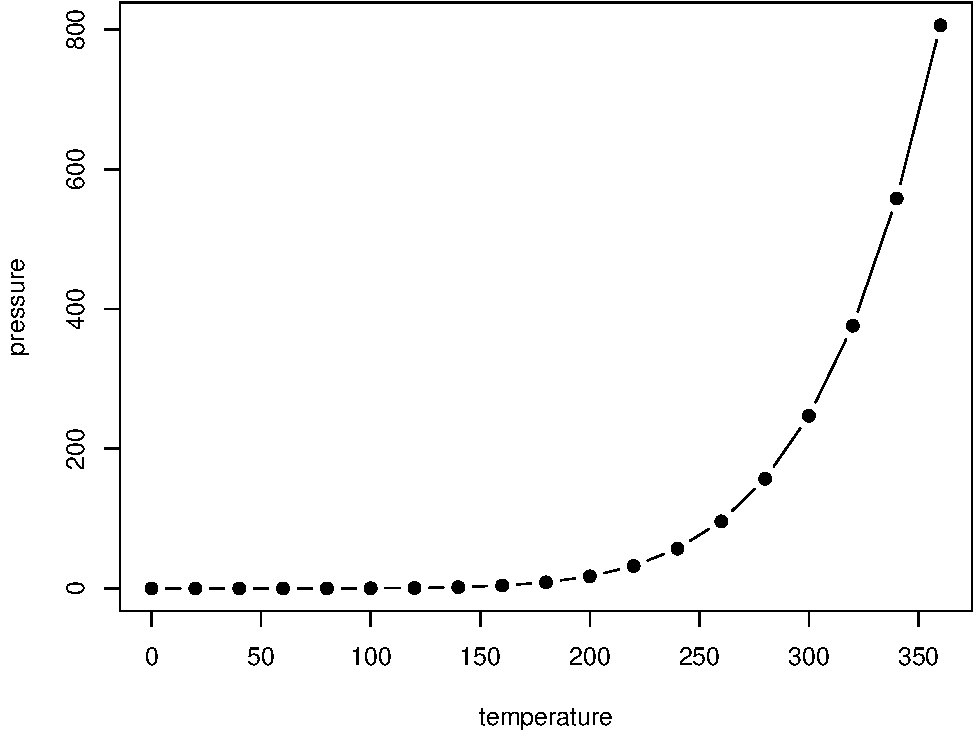
\includegraphics[width=0.8\linewidth]{BookRepTemplates_files/figure-latex/nice-fig-1} 

}

\caption{Here is a nice figure!}\label{fig:nice-fig}
\end{figure}

Reference a figure by its code chunk label with the \texttt{fig:}
prefix, e.g., see Figure \ref{fig:nice-fig}. Similarly, you can
reference tables generated from \texttt{knitr::kable()}, e.g., see Table
\ref{tab:nice-tab}.

\begin{table}

\caption{\label{tab:nice-tab}Here is a nice table!}
\centering
\begin{tabular}[t]{rrrrl}
\toprule
Sepal.Length & Sepal.Width & Petal.Length & Petal.Width & Species\\
\midrule
5.1 & 3.5 & 1.4 & 0.2 & setosa\\
4.9 & 3.0 & 1.4 & 0.2 & setosa\\
4.7 & 3.2 & 1.3 & 0.2 & setosa\\
4.6 & 3.1 & 1.5 & 0.2 & setosa\\
5.0 & 3.6 & 1.4 & 0.2 & setosa\\
\addlinespace
5.4 & 3.9 & 1.7 & 0.4 & setosa\\
4.6 & 3.4 & 1.4 & 0.3 & setosa\\
5.0 & 3.4 & 1.5 & 0.2 & setosa\\
4.4 & 2.9 & 1.4 & 0.2 & setosa\\
4.9 & 3.1 & 1.5 & 0.1 & setosa\\
\addlinespace
5.4 & 3.7 & 1.5 & 0.2 & setosa\\
4.8 & 3.4 & 1.6 & 0.2 & setosa\\
4.8 & 3.0 & 1.4 & 0.1 & setosa\\
4.3 & 3.0 & 1.1 & 0.1 & setosa\\
5.8 & 4.0 & 1.2 & 0.2 & setosa\\
\addlinespace
5.7 & 4.4 & 1.5 & 0.4 & setosa\\
5.4 & 3.9 & 1.3 & 0.4 & setosa\\
5.1 & 3.5 & 1.4 & 0.3 & setosa\\
5.7 & 3.8 & 1.7 & 0.3 & setosa\\
5.1 & 3.8 & 1.5 & 0.3 & setosa\\
\bottomrule
\end{tabular}
\end{table}

You can write citations, too. For example, we are using the
\textbf{bookdown} \index{bookdown} package \citep{R-bookdown} in this
sample book, which was built on top of R Markdown \index{R Markdown} and
\textbf{knitr} \index{knitr} \citep{xie2015}.

\chapter{Literature}\label{literature}

Here is a review of existing methods.

\part{Part Two}\label{part-part-two}

\chapter{Methods}\label{methods}

We describe our methods \index{Some Methods} in this chapter.

add more random text \index{text}.

\chapter{Applications}\label{applications}

Some \emph{significant} applications are demonstrated in this chapter.

\section{Example one}\label{example-one}

\section{Example two}\label{example-two}

\chapter{Final Words}\label{final-words}

We have finished a nice book \index{Nice Book}.

some random \index{random} text

\bibliography{manual.bib,packages.bib}

\printindex


\end{document}
